\documentclass[a4paper,
fontsize=11pt,
%headings=small,
oneside,
numbers=noperiodatend,
parskip=half-,
bibliography=totoc,
final
]{scrartcl}

\usepackage{synttree}
\usepackage{graphicx}
\setkeys{Gin}{width=.4\textwidth} %default pics size

\graphicspath{{./plots/}}
\usepackage[ngerman]{babel}
\usepackage[T1]{fontenc}
%\usepackage{amsmath}
\usepackage[utf8x]{inputenc}
\usepackage [hyphens]{url}
\usepackage{booktabs} 
\usepackage[left=2.4cm,right=2.4cm,top=2.3cm,bottom=2cm,includeheadfoot]{geometry}
\usepackage{eurosym}
\usepackage{multirow}
\usepackage[ngerman]{varioref}
\setcapindent{1em}
\renewcommand{\labelitemi}{--}
\usepackage{paralist}
\usepackage{pdfpages}
\usepackage{lscape}
\usepackage{float}
\usepackage{acronym}
\usepackage{eurosym}
\usepackage[babel]{csquotes}
\usepackage{longtable,lscape}
\usepackage{mathpazo}
\usepackage[flushmargin,ragged]{footmisc} % left align footnote

\usepackage{listings}

\urlstyle{same}  % don't use monospace font for urls

\usepackage[fleqn]{amsmath}

%adjust fontsize for part

\usepackage{sectsty}
\partfont{\large}

%Das BibTeX-Zeichen mit \BibTeX setzen:
\def\symbol#1{\char #1\relax}
\def\bsl{{\tt\symbol{'134}}}
\def\BibTeX{{\rm B\kern-.05em{\sc i\kern-.025em b}\kern-.08em
    T\kern-.1667em\lower.7ex\hbox{E}\kern-.125emX}}

\usepackage{fancyhdr}
\fancyhf{}
\pagestyle{fancyplain}
\fancyhead[R]{\thepage}

%meta
%meta

\fancyhead[L]{Chr.Szepanski \\ %author
LIBREAS. Library Ideas, 27 (2015). % journal, issue, volume.
\href{http://nbn-resolving.de/urn:nbn:de:kobv:11-100229855
}{urn:nbn:de:kobv:11-100229855}} % urn
\fancyhead[R]{\thepage} %page number
\fancyfoot[L] {\textit{Creative Commons BY 3.0}} %licence
\fancyfoot[R] {\textit{ISSN: 1860-7950}}

\title{\LARGE{Ein Blick auf das Davor. Metatheorien am Beispiel der Activity Theory in der Informationsverhaltensforschung}} %title %title
\author{Christoph Szepanski} %author

\setcounter{page}{36}

\usepackage[colorlinks, linkcolor=black,citecolor=black, urlcolor=blue,
breaklinks= true]{hyperref}

\date{}
\begin{document}

\maketitle
\thispagestyle{fancyplain} 

%abstracts

%body
\section*{Der Methode voraus --
Metatheorien}\label{der-methode-voraus-metatheorien}

Im enzyklopädisch angelegten Sammelband verschiedener Theorien, Methoden
und Praktiken der Informationsverhaltensforschung von Karen E. Fisher et
al. findet sich eine recht knappe Einführung von Marcia J. Bates (2005:
10-14) zu den dreizehn gebräuchlichsten Metatheorien\footnote{\emph{Metatheorien}
  beinhalten Aussagen über Theorie, geben an, welche Begriffe
  hinzugezogen werden sollten und wie sie miteinander in Beziehung zu
  setzen sind. (Bates 2005: 2)} der Library and Information Science
(LIS). Sie seien hier in alphabetischer Reihenfolge kurz wiedergegeben:

\begin{itemize}
\itemsep1pt\parskip0pt\parsep0pt
\item
  bibliometric
\item
  cognitive
\item
  constructionist
\item
  constructivist
\item
  critical theory
\item
  engineering
\item
  ethnographic
\item
  evolutionary
\item
  historical
\item
  philosophical-analytic
\item
  socio-cognitive
\item
  user-centered design
\end{itemize}

Auffällig ist hierbei, dass nahezu alle Metatheorien aus anderen Fächern
importiert wurden und lediglich die Bibliometrie als der LIS inhärenten
Metatheorie bewertet werden kann. Dies muss nun nicht gleich schlecht
sein.

Es war schon immer Realität, dass kleinere Fächer kaum eigene
Theoriearbeit leisten konnten und auf Impulse von anderen Disziplinen
angewiesen waren. Eine weitere Rolle hinsichtlich des Zustands der
Theoriebildung und Methodendiskussion im Fach LIS spielt sicher auch der
Umstand, dass das Studium per se auf einen relativ fest umrissenen
Berufsstand mit verhältnismäßig klaren Tätigkeitsfeldern vorbereiten
soll. Es erscheint aus dieser Perspektive zeckmäßig, dass die
Auseinandersetzung mit eher praxisnahen Gegenständen wie
Recherchefähigkeiten, Kennzahlenverständnis, die Beherrschung der
aktuellen EDV und einiger Programmiersprachen, Managementtechniken oder
das Befassen mit Implementierungsfragen in der Ausbildung und im
späteren Berufsleben richtigerweise im Vordergrund steht. Ist jedoch
Wissen über informationswissenschaftlich relevante Theorien und Methoden
nicht ebenso wichtig für die Praxis, um beispielsweise Komplexität
bewältigen zu können?

Anhand des holistischen Ansatzes der Activity Theory (AT)\footnote{Die
  Activity Theory kann den soziokognitiven Metatheorien zugeordnet
  werden.} soll in diesem Beitrag für mehr theoretische Substanz in
Studien der Informationsverhaltensforschung argumentiert werden. An
einigen Stellen wird mit einer generellen Übertragbarkeit der
Argumentation für die gesamte Informationswissenschaft kokettiert. Im
weiteren Verlauf wird die AT kurz vorgestellt, das derzeitige
methodische Profil von Studien aus der Informationsverhaltensforschung
skizziert und zwei aktuelle Untersuchungen aus der AT-Forschung
besprochen. Am Ende wird der Frage nachgegangen, ob sich die Activity
Theory mit dem informationswissenschaftlichen Fundus vereinen lässt.

\section*{Die Situation in der
Informationsverhaltensforschung}\label{die-situation-in-der-informationsverhaltensforschung}

Die Informationsverhaltensforschung verfügt über ein breites, jedoch
wenig theoretisch abgesichertes Methodenwissen. Zwei Ansätze aus den
Anfängen dieses Teilgebietes erleben einen ständig wiederkehrenden Hype
und sind vielleicht aktueller denn je.

Zum einen handelt es sich um George Zipfs \enquote{Principle of Least
Effort (PLE)} (1949), das besagt, dass Menschen den Aufwand für
Handlungen im Rahmen einer stetigen Kosten-Nutzen-Rechnung abwägen, was
aus dieser Perspektive nachvollziehbar, auch auf den Umgang mit
Informationen zutrifft. Dieser Gedanke wird in Peter Pirollis
\enquote{Information Foraging Theory} (1999) aufgenommen und vor allem
im Hinblick auf die Informationssuche weiterentwickelt. Pirolli
verknüpft Zipfs PLE mit George Millers Ansatz des
\enquote{Informavores}\footnote{Miller entwickelte hier die Theorie des
  Menschen als informationsverbrauchenden Organismus.} und behauptet
Menschen nähmen die Welt vor allem durch das Suchen und Nutzen von
Informationen wahr, deren Produkt die Grundlage für Entscheidungen
bildet.

Menschen sind, so behauptet Miller, informationsverbrauchende Organismen
und wägen -- ähnlich wie Tiere bei der Nahrungssuche -- die
Beschaffungskosten für neue Informationen und Wissen ab und sind bereit,
auf möglicherweise gewinnbringende Informationen zu verzichten, wenn der
Aufwand situativ als zu groß erscheint.\footnote{Hier beispielsweise die
  Recherche in einem Informationssystem.} Verantwortlich sei hierfür das
\enquote{Information Scent Module}, worin zuvor genannte
Kosten-Nutzen-Abwägungen angestellt werden ( Hobohm 2013: 113).
Flankiert wird diese recht rationale Abwägung über den Informationswert
von sozialen Faktoren, vergleichbar ähnlich der Pheromonspur bei
Ameisen, die Pirolli mit \enquote{Information Scent} beschreibt. So kann
Pirollis \enquote{Information Foraging} zumindest nachvollziehbar
gestalten, warum Menschen in Informationssystemen häufig nicht über die
ersten Treffer hinaus \emph{jagen} und insbesondere in Zeiten von Social
Media Informationen, die von anderen Menschen als relevant eingestuft
wurden, -- \emph{die Beute} sozusagen -- bevorzugen oder ihnen einen
subjektiv höheren Wert verleihen.

Verfahren wie Googles Page Rank, Amazons Recommender System oder auch
der Impact Factor scheinen sich aus diesen Beobachtungen einen Vorteil
zu verschaffen. Eine hierzu naheliegende Vorhersage wäre, dass
fortwährend diejenigen Informationssysteme und -umwelten bevorzugt
werden, die diese scheinbar tief in uns verankerten evolutionären
Verfahrensweisen bezüglich der Informationsverarbeitung bedienen. Eine
weitere Beobachtung ist, die diese Theorie stützt, dass die Menschen in
modernen Gesellschaften erheblich mehr Zeit damit verbringen,
Informationen finden zu wollen, Daten zu konsumieren oder sich in
Informationsumwelten einfach nur treiben zu lassen. Die eigentliche,
lebenswichtige Nahrungssuche erfolgt in hochentwickelten Gesellschaften
zunehmend nachgeordnet. Marian Dörk et al. widmen sich aus dieser
Perspektive des \enquote{Information Flaneur} heraus der ungerichteten
Informationssuche und liefern hier wichtige Impulse für das Interface
Design (Dörk et al. 2011: 1222).

Metaphorisch ausgedrückt: Wo damals auf Ziegen gestarrt wurde, starren
wir heute auf Bildschirme und lassen uns solange vom bunten Treiben
fesseln, bis sich genügend Erfolgsmomente eingestellt haben oder eine
Steigerung nicht mehr möglich ist -- wir nicht mehr das Gefühl haben,
ähnlich wie poikilotherme Tiere, \emph{wärmer} zu werden.\footnote{In
  Anlehnung an Jakob Nielsens Metapher: \enquote{Informavores will keep
  clicking as long as they sense (to mix metaphors) that they're getting
  warmer -- the scent must keep getting stronger and stronger, or people
  give up.}, unter anderem nachgewiesen hier:
  \url{http://www.nngroup.com/articles/information-scent/}}

\begin{quote}
\enquote{Heute leben wir im Imaginären des Bildschirms, des Interface
und der Vervielfältigung, der Kommunikation und Vernetzung. Alle unsere
Maschinen sind Bildschirme, wir selber sind Bildschirme geworden und das
Verhältnis der Menschen zueinander ist das von Bildschirmen geworden.}
(Jean Baudrilliard 1992: 263)
\end{quote}

Sergei L. Rubinstein, bedeutender Vertreter der sowjetischen
kulturhistorischen Schule, war Mitte der 1920er Jahre der Ansicht, dass
(gegenständliche) Handlungen nicht nur Einfluss auf die Umwelt haben,
sondern ebenso den Akteur selbst beeinflussen würden (vgl. auch Häyrynen
1999: 120; Wilson 2006: online). Über die Kybernetik fand diese
Perspektive schließlich in die heutigen Neurowissenschaften Eingang, die
die Ansicht vertreten, dass sich durch Handeln die Struktur des Gehirns
ständig neu organisiert. Hier kann die Brücke zur \enquote{Information
Foraging Theory} geschlagen werden, wenn dies als evolutionärer Prozess
verstanden wird, um weiterhin effizient im Rahmen der täglichen
Informationsjagd funktionieren zu können. Dieser Prozess hat, so die
These, ausdrücklich keine langfristigen negativen Effeke auf das Gehirn
zu Folge, wie zum Beispiel von Manfred Spitzer behauptet. Spitzer legt
es unverständlicherweise negativ aus, dass Instrumente, die uns den
Prozess der Externalisierung\footnote{Externalisierung beschreibt die
  Neuentwicklung, beziehungsweise Transformation menschlich geschaffener
  Instrumente (A\emph{rtefakte).}} erleichtern, immer Einfluss auf unser
Sein haben. Die Entstehungs- und Nutzungsgeschichte des Menschen und
seinen Instrumenten, angefangen über den Faustkeil bis hin zum
Hipsteraccessoire der Uhr mit integriertem Taschenrechner oder dem
Smartphone, wo Subjekt, Instrument und Objekt oft miteinander
verschmelzen zu scheinen, bestätigen diese Annahme jedoch nicht.

Die AT\footnote{In deutschsprachigen Raum ist sie unter dem Begriff
  Tätigkeitstheorie bekannt.} reiht sich im Kanon dieser Behauptungen
ein, wenn sie unterstellt, Techniken und Maschinen würden nicht nur vom
Menschen geschaffen sein, sondern auch der Mensch selbst wird von seinen
geschaffenen Objekten bestimmt (vgl. Kaptelinin und Nardi 2012). Dadurch
erweitert sich der Kontext menschlichen Informationsverhaltens enorm, da
hier die Entwicklungs- und Nutzungsgeschichte von Artefakten
Berücksichtigung findet. Die vom Menschen geschaffenen Gegenstände
würden schließlich die Erfahrungen von Akteuren reflektieren, die vor
ähnlichen Problemen standen, so ein gängiger tätigkeitstheoretischer
Ansatz.

Ein Blick in die letzten Untersuchungen zu den \emph{Trends} in der
Informationsverhaltensforschung gibt einiges mehr zu erkennen. Während
laut Pertti Vakkari (1993, 2008) der Anteil rein Theorie geleiteter
Forschungen stetig zunahmen und um die Jahrtausendwende anteilig ihren
Höhepunkt erreichte (Pettigrew 2001), kann zumindest in der von Elke
Greifeneder (2014) durchgeführten aktuellen Untersuchung festgehalten
werden, dass solche Verfahren einen festen Platz in der
informationswissenschaftlichen Publikationskultur zur
Informationsverhaltensforschung einnehmen, auch wenn solcherart Studien
dennoch rückläufig sind.

Greifeneder fand zudem heraus, dass der Anteil in der Verwendung von
Mischtechniken (Mixed Methods) bei 45\% lag (n=155), wobei 7\% der
Studien mehr als zwei Methoden einsetzten und die Methodenvielfalt
insgesamt zunähme. Qualitative Methoden, vor allem Interviews,
überwiegen. Selbst vor dem Hintergrund bisher wenig bearbeiteter
Forschungsfelder wie die Informationsnutzung mittels mobiler Endgeräte
oder die Erforschung von Informationsbedürfnissen von besonderen
Personengruppen, wie beispielsweise Drogenabhängige oder
Personengruppen, welche Schicksalsschläge verarbeiten müssen,\footnote{Unter
  dem Titel \enquote{A Shared Space and a Space for Sharing: A
  Transdisciplinary Exploration of Online Trust and Empathy} versucht
  die britische University of Sheffield in Rahmen eines
  Forschungsprojektes diese Frage zu beantworten. Für weitere
  Informationen siehe dazu:
  \url{https://www.sheffield.ac.uk/is/research/projects/sharedspace}
  (06.05.2015)} dürfte die zukünftige Methodenwahl in diesem Teilgebiet
wenig verändern, da wie bereits durch diese beiden Beispiele impliziert,
die Zukunft eher im \enquote{Information Seeking}, als in der
Gesamtbetrachtung menschlichen Informationsverhaltens liegt (vgl. auch
Vakkari 2008: online). Greifeneder schätzt zudem die Chancen einer
möglichen Meta-Diskussion über die Methodenwahl in der (nahen) Zukunft
erwartungsgemäß als gering ein.

Abschließend und soweit sich das nach Sichtung der Literatur beurteilen
lässt, unterteilen sich die Akteure der Informationsverhaltensforschung
weiterhin in zwei große Lager: erstere versuchen aus einer holistischen
Perspektive heraus mit klaren theoretischen Bezügen menschliches
Informationsverhalten begreifbar zu machen, während die zweite große
Gruppe sich oft ohne größere theoretische Bezüge in Form eines
\emph{Schnappschusses} Teilproblemen widmet (vgl. Fidel 2012: 148;
Wilson 2006: online). Grundsätzlich, soweit ersichtlich, bedarf es
jedoch ein \emph{Mehr} an zusammenführenden Theorien, die dabei helfen
die jeweilige Methodenwahl zu begründen.

Auf absehbare Zeit wird sich, so eine Einschätzung, daran wenig ändern.
Wie Ben Kaden und Karsten Schuldt im Rahmen eines Informare!-Workshops
erörterten (2012), ist in informationswissenschaftlichen Kreisen eher
wenig intrinsisches Interesse an aktiver Interdisziplinarität
beobachtbar, was unter anderem darin mündet, dass beispielsweise
Konzepte zur Steigerung von Informationskompetenz oftmals am breiten
Fundament der pädagogischen Forschung scheuklappenhaft vorbei entwickelt
werden. Sylvain Cibangu stuft hierzu auch den kaum vorhandenen
innerdisziplinären informationswissenschaftlichen Austausch als
problematisch ein (2013: 204).

\section*{Ein Exot in Gestalt eines Dreieckes betritt den Raum:
Activity
Theory}\label{ein-exot-in-gestalt-eines-dreieckes-betritt-den-raum-activity-theory}

Ihren Ursprung hat die AT in der kulturhistorischen Schule der
Sowjetunion der 1920er und 1930er Jahre. Konzipiert wurde sie, um die
Entstehung des Wissens und deren Vermittlung fundierter beschreiben zu
können, wobei anfangs Kinder und Jugendliche im Fokus standen.
Spätestens mit der dritten Welle der AT-Forschung, Mitte der 1980er
Jahre, wurde es zur gängigen Praxis, tätigkeitstheoretische Überlegungen
über eine Dreiecksstruktur\footnote{Häufig wird hierfür auch der Begriff
  \enquote{Tätigkeitssystem} verwendet.} einzuführen. In diesem Zeitraum
fällt auch die Verlagerung des Schwerpunkts weg von lerntheoretischen
Überlegungen hin zur Arbeits- und Koorperationsforschung (Kumbruck 2001:
151).

Zentrales Definitionselement bildet das \emph{Objekt der Tätigkeit},
häufig auch mit \emph{Gegenstand der Tätigkeit} oder \emph{Produkt}
beschrieben. Yrjo Engeström (1987) behauptet, dass jedes
Tätigkeitssystem, nur ein Objekt beinhaltet, auf das alle Akteure
motivational ausgerichtet sind und mit ihren Tätigkeiten folglich darauf
einwirken. Selbstverständlich kann es in Organisationen oder -- eine
Ebene niedriger gedacht -- hinsichtlich Kollaborationen verschiedene
Objekte geben, die dann entsprechend in mehrere Tätigkeitssysteme
aufzuteilen sind. Weiterhin besteht ein Tätigkeitssystem aus den
Elementen \emph{Subjekt}, \emph{Instrumente}, \emph{Arbeitsteilung},
\emph{Gemeinschaft} und \emph{Regeln} (Hackel und Klebl 2008: 3). Jene
Elemente stehen untereinander im kontinuierlichen Austausch, bedingen
und konstruieren einander. Seit Anfang der 2000er Jahre liegt der Fokus
auf verschiedene Tätigkeitssysteme, die in Netzstrukturen analysiert
werden. Behindern sich benachbarte und miteinander vernetzte
Tätigkeitssysteme gilt es die Ursachen für ein solche Barriere
(Widersprüche) zu identifizieren und wenn möglich die Transformation in
ein gemeinsames Tätigkeitssystem zu verfolgen, um die Tätigkeit an sich
weiterzuentwickeln.

Paulo Barthelmess und Kenneth M. Anderson ist es gelungen, die zuvor
dargelegte tätigkeitstheoretische Perspektive überaus kompakt
zusammenzufassen:

\begin{quote}
To summarize, activities are performed by subjects, motivated by a goal,
transforming an object into an outcome. An object may be shared by a
community of actors, that work together to reach a desired outcome.
Tools, rules and division of labor mediate the relationship between
subjects, community and object. Activities are carried out by actions,
which in turn are realized as sets of operations." (Barthelmess und
Anderson 2002: 17)
\end{quote}

Obwohl in den letzten zehn Jahren relativ intensiv, vor allem
international, bearbeitet (Wilson 2006; Widen-Wulff und Davonport 2007;
Allen 2011; Roos 2012; Isah und Byström 2015), findet sich bis auf
wenige Bruchstücke in den aktuellen deutschsprachigen Handbüchern wie
den \enquote{\emph{Grundlagen der praktischen Information und
Dokumentation}} (Kuhlen et al. 2013) oder dem \enquote{\emph{Handbuch
Methoden der Bibliotheks- und Informationswissenschaft}} (Umlauf et al.
2013) nichts zur AT. Für die LIS des deutschsprachigen Raums ist sie
infolgedessen nicht einmal in die Kategorie eines Randthemas einzuordnen
und auch alles andere als \emph{hipster}. Das Ergebnis für
deutschsprachige Zeitschriften wie die \emph{Information, Wissenschaft
und Praxis} fällt ähnlich aus.

Über die Ursache hierfür kann bestenfalls spekuliert werden, dies wäre
jedoch allemal eine ausführliche Auseinandersetzung in einem eigenen
Artikel wert. Ein Problem ist sicher, dass der überwiegende Teil an
Studien aus dem Bereich der Informationsverhaltensforschung einer
Momentaufnahme -- eines Schnappschusses -- wie es Thomas Wilson (2006)
oder Raya Fidel (2012: 148) formulierten, gleicht. Auf der anderen Seite
bestehen keinerlei Einwände darüber, dass sich solcherart
systemorientierte Ansätze, wie hier beschrieben, ungleich schwerer
operationalisieren lassen und in Folge des Forschungsalltages durchaus
mehr Zeit für ein solches Vorhaben aufgewendet werden müsste, wobei
unklar ist, ob die Ergebnisse am Ende über Allgemeinplätze hinaus gehen
könnten.

\begin{figure}[htbp]
\centering
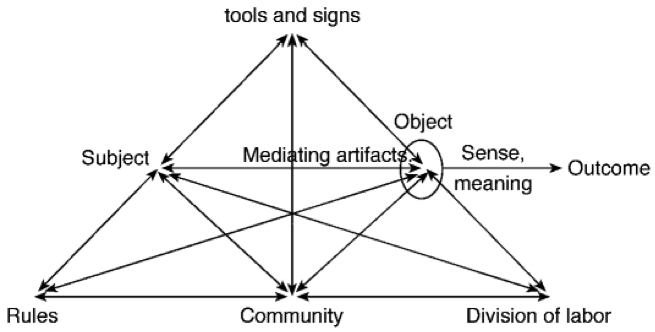
\includegraphics{img/abbildung1.png}
\caption{Engeströms human activity system. (2001: 135)}
\end{figure}

Dies führt letztlich zu der These, dass Akteure nicht nur in Bezug auf
die \emph{Jagd nach neuen Informationen} bereit sind auf diese zu
verzichten, wenn ihnen der Aufwand als zu groß erscheint und ihre
Wissensbasis zur Bewältigung alltäglicher Herausforderungen und
Problemstellungen ausreicht, sondern auch auf die Wahl der Instrumente,
wenn diese zur Beantwortung von Phänomenen augenscheinlich genügen.
Selbst innerhalb der AT-Forschung herrschen große Unterschiede, die
Operationalisierung sowie intensive Auseinandersetzung und Befolgung
tätigkeitstheoretischer Überlegungen betreffend, wie Amanda Quek und
Hanifa Shah (2004) nachwiesen.

Zwei tätigkeitstheoretische Studien, deren Operationalisierung als
gelungen zu werten sind, sollen hier kurz wiedergegeben werden. Die
erste handelt von der Informationspraxis von Molekularmedizinern und
stammt von Anniki Roos (2012). Unter der Prämisse, holistische Forschung
erschiene zunehmend lohnenswerter im Rahmen
informationswissenschaftlicher Untersuchungen, da Informationsumwelten
selbst komplexer würden und lediglich die ganzheitliche Perspektive den
neuen Anforderungen gewachsen sein könnte, nutzt sie hier AT als
Instrument, um zunächst die Komplexität molekularmedizinischer Forschung
zu strukturieren. Anschließend kombinierte sie die
tätigkeitstheoretische Perspektive mit Birger Hjørlands \enquote{Domain
Analysis} (1995). Diese Theorie geht davon aus, Information wäre
letztlich nur im Kontext der ihr zugrundeliegenden Wissensorganisation,
der Sprache, den eingesetzten Kommunikationsmitteln und
Informationssystemen zu verstehen und wäre insgesamt eine Reflexion auf
die gesellschaftliche Rolle der gegenständlichen Tätigkeit mitsamt deren
Objekt(en) (Roos 2012: online). Sie erhoffte sich dadurch ein
tiefergreifendes Verständnis in Bezug auf die Nutzung und
problemlösungsorientierte Suche nach Informationen seitens der
Mediziner, weshalb sie auch Befragungen durchführte.

Roos schildert die Informationsumwelt von Molekularmedizinern als
datenintensiv, welche geprägt ist in wiederkehrenden, längeren
Recherchen in vorzugsweise medizinischen Datenbanken wie PubMed und die
Benutzung von Software beispielsweise zur Datenauswertung oder
Berechnung von Modellen. Des Weiteren ist die Arbeit gekennzeichnet von
einem relativ strukturierten Forschungsalltag (vgl. dazu Abb. 4, Roos
2012: online). Sie identifiziert Recherchetätigkeiten als nachrangig zu
bewertende Handlungen, die nur einen kleinen Teil der eigentlichen
Forschungsalltags von Molekularmedizinern einnehmen würden. Sie
interpretiert dies als einen Hinweis für die recht geringe Nutzung der
bibliothekarischen Angebote und deutet an, die hiesigen
\enquote{Information Professionals} könnten die Mediziner am ehesten
durch die Entwicklung komfortabler zu nutzender Interfaces,
Filterfunktionen oder enger vernetzten Schnittstellen zwischen den
Informationsmitteln und weniger mit Initiativen, die auf eine
persönlicheren Kontakt (\emph{embedded}) mit den Forschern hinauslaufen,
unterstützen.

\begin{figure}[htbp]
\centering
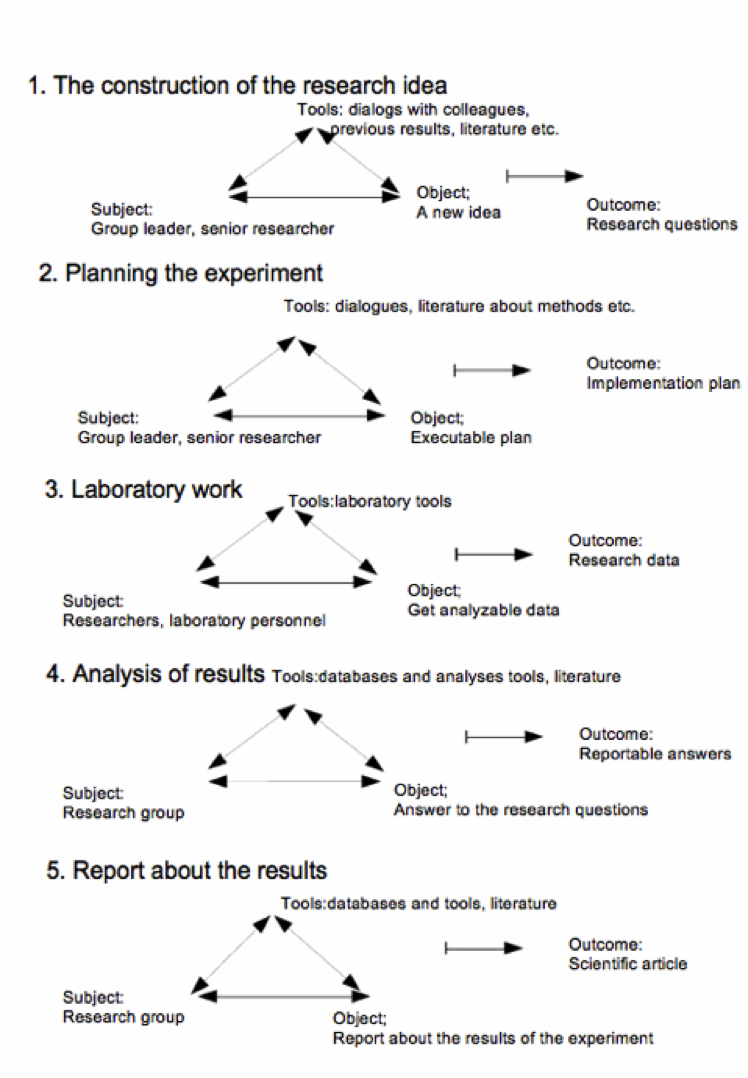
\includegraphics{img/abbildung2.png}
\caption{Handlungskette molekularmedizinischer Forschungsaktivität.
(Roos 2012: online)}
\end{figure}

Die zweite Studie von Judith Brown et al. (2013) legt den Fokus auf die
Erfassung und Strukturierung der in einem \enquote{großen Datencenter}
beobachteten Tätigkeiten. Neben der Beobachtung wurde auch mit
halbstrukturierten Interviews gearbeitet (n=10), die sich an der
\enquote{Activity Checklist} orientierten (vgl. Kaptelinin et al. 1999).
Aufgabe dieser Einrichtung war das Customer-Relationship-Management. In
einem zweiten Schritt wurden Widersprüche identifiziert, die die Arbeit
intraorganisational behindern.

Zum einen konnte die Forschergruppe sichtbar machen, dass teils
veraltete IT wie das Ticket-System, Arbeitsabläufe künstlich
komplizierter gestalten würde, beispielsweise würden zu lange
Schilderungen innerhalb eines einzigen Tickets die Mitarbeiter oft
überfordern und das Management von mehreren \emph{bridge calls} sei
fehlerfrei nur schwer möglich zu realisieren. Zum anderen würden die
Räumlichkeiten face-to-face Kommunikation behindern und so einen
effektiveren Arbeitsablauf behindern. Neben einigen weiteren
Optimierungsmöglichkeiten, machen die Autoren jedoch auf einen wichtigen
Punkt hinsichtlich des Studiendesigns aufmerksam: viele der im
Datencenter herrschenden Widersprüche wären in Laborsituationen oder
anders konzipierten Feldstudien folglich nur sehr schwer zu
reproduzieren gewesen (Brown et al. 2013: 273).

Tätigkeitstheoretische Forschung dürfe deshalb nicht allein \enquote{am
Desktop} geschehen (vgl. Quek und Shah 2004: 7; Wilson 2008: 139),
sondern müsse zwingend den Weg in die Praxis finden.

\section*{Don't be square! Versuch einer Argumentation für mehr
Activity Theory in der
Informationswissenschaft}\label{dont-be-square-versuch-einer-argumentation-fuxfcr-mehr-activity-theory-in-der-informationswissenschaft}

Es ist erstaunlich wie leichtfüßig sich tätigkeitstheoretische
Überlegungen mit dem informationswissenschaftlichen Fundus verknüpfen
lassen, schließlich müssen sich Metatheorien laut Brian Campbell Vickery
für eine Vielzahl von in der LIS bearbeiteten Gegenständen als fruchtbar
erweisen (Vickery 1997: 458). Denkbar wäre neben der jetzt schon
wiederkehrenden Anwendung in der Informationsverhaltensforschung der
(internationalen) LIS, ebenso eine intensivere Beschäftigung im Rahmen
des Qualitätsmanagements von Informationsservices oder beispielsweise
der Informationskompetenzforschung. Hier könnte, neben der
lerntheoretischen Perspektive der AT, durchaus auch die
interdisziplinäre Bearbeitung tätigkeitstheoretischer Gegenstände
helfen, allen voran in der Psychologie, der Informatik und eben der
Pädagogik. Hilfreich ist hier sicher die weitestgehend interdisziplinäre
Übereinstimmung über Basiselemente und -prinzipien der AT (Widen-Wulff
und Davenport 2007: online) und die minimalere Kontextdimension des
Tätigkeitssystems, im Vergleich zu einem abstrakten gesellschaftlichen
System, was jedoch nichtsdestotrotz die Auseinandersetzung mit komplexen
Organisationen und Formen der Kollaboration zulässt. So ist
beispielsweise die Wikipedia nicht nur im Sinne des
tätigkeitstheoretischen Vokabulars als \emph{Instrument}, sondern auch
als \emph{Gemeinschaft} zu verstehen -- eine Perspektive, die sich auch
bei Clay Shirky finden lässt (2008: 136).

Des weiteren wird dafür plädiert, sich der impliziten Wissensdimension
(Polanyi 1985) nicht länger über den Handlungsbegriff, sondern über die
dreiteilige hierarchische Struktur der Tätigkeit zu nähern. Im Gegensatz
zur viel bewusster und zielgerichteten Auslegung von Handlungen, umfasst
Tätigkeit auch die nicht expliziten und nicht explizierbaren Aspekte
menschlicher Tätigkeit. Die CSCW-Forschung, das Konzept der Communities
of Practice (Zboralski 2007) sowie Ikujiro Nonaka und Hirotaka Takeuchi
mit ihrem SECI-Modell,\footnote{Die ``Wissensspirale oder auch
  SECI-Prozess (Socialisation, Externalisation, Combination and
  Internalisation). Nonaka und Takeuchi gingen hier den so wichtigen
  Schritt Wissen nicht mehr als objektive Entität zu betrachten, sondern
  als einen sozialen Konstruktionsprozess. Das Werk prägte vor allem die
  zweite Generation des Wissensmanagements.} widmen sich dem impliziten
Wissen hinsichtlich schwer zu erfassender kollektiver Aktivität. Die AT
könnte hier ebenfalls Anwendung finden, da sie sich ebenso
Fragestellungen zum schwer antizipierbaren, situierten Handeln widmet
und die Mitmenschen als Teil des Kontextes begreift, auf den sich die
Akteure einstellen.

Nardi (1996: 90-95) argumentiert ausdrücklich für eine
abwechslungsreiche, um nicht zu sagen experimentelle Methodengestaltung,
hinsichtlich tätigkeitstheoretischer Untersuchungen. Es sei hier
ausdrücklich darauf hingewiesen, dass die AT nicht nur als Metatheorie
zu verstehen ist, sondern auch Instrumente zur Analyse mitliefert (vgl.
Korpela 1997; Kaptelinin 1999).

Abschließend kann hier insgesamt nur für eine energische
Auseinandersetzung mit theoretischen Bezügen appelliert werden, die sich
dann hoffentlich sichtbarer in der Methodenwahl und -diskussion
wiederfinden. Ausbildung sowie das spätere Berufsleben müssen hier
Möglichkeiten schaffen, Theorie und Praxis enger miteinander zu
verzahnen, um das Fach mit Kollektiven an \enquote{Theory-illumined
Practioner} (Cibangu 2013: 207) zu versorgen.

\section*{Literatur}\label{literatur}

ALLEN, David (2011): Information Behavior and Decision Making in
Time-Constrained Practice: A Dual-Processing Perspective. In: JASIST, 62
(11). S.2165-2181.

BATES, Marcia J. (2005): An Introduction to Metatheories, Theories and
Models. In: Fisher, Karen E.; Erdelez, Sandra und McKechnie, Lynne
(Hrsg.): Theories of Information Behavior. Cambridge, Mass. : MIT Press.
S.1-24.

BARTHELMESS, Paulo; Anderson, Kenneth M. (2002): A view of Software
Development Environments based on Activity Theory. In: CSCW, 11.
S.13-37.

BAUDRILLARD, JEAN (1992): Aisthesis. Wahrnehmung heute oder Perspektiven
einer anderen Ästhetik. Leipzig : Reclam.

BROWN, Judith M; GREENSPAN, Steven und BIDDLE, Robert (2013): Complex
activities in an operations center: a case study and model for
engineering interaction. In: Proceedings of EICS. S.265-274.

CASE, Donald O. (2005): Principle of Least Effort. In: Fisher, Karen E.;
Erdelez,Sandra und McKechnie, Lynne (Hrsg.): Theories of Information
Behavior. Cambridge, Mass. : MIT Press. S.289-292.

ENGESTRÖM, Yrjö (1987): Learning by expanding: An activity-theoretical
approach to developmental research. Helsinki : Orienta Konsulit.

CIBANGU, Sylvain K. (2013): A memo of qualitative research for
information science: toward theory construction. In: JoD, 69 (2).
S.194-213.

DÖRK, Marian; CARPENDALE, Sheelagh und WILLIAMSON, Carey (2011):
\href{http://mariandoerk.de/informationflaneur/chi2011.pdf}{The
Information
Flaneur:}\href{http://mariandoerk.de/informationflaneur/chi2011.pdf}{A
Fresh Look at Information Seeking}. In: CHI 2011: Proceedings of the
SIGCHI Conference on Human Factors in Computing Systems, ACM.
S.1215-1224.

ENGESTRÖM, Yrjö (2001): Expansive Learning at Work: toward an activity
theoretical reconceptualization. In: Journal of Education, 14 (1).
S.133-156. DOI: 10.1080/13639080020028747.

FIDEL, Raya (2012): Human Information Interaction: An Ecological
Approach to Information Behavior. Cambridge {[}u.a.{]} : MIT Press.

GREIFENEDER, Elke (2014): Trends in information behaviour research. In:
\emph{Proceedings of ISIC, the Information Behaviour Conference}. Leeds,
2-5 September, 2014: Part 1.
\url{http://www.informationr.net/ir/19-4/isic/isic13.html}

HÄYRYNEN, Yrjö-Paavo (1999): Collapse, creation and continuity in
Europe: how do people change? In: Engeström, Yrjö; Miettinen, Reijo und
Punamäki, Raija L. (Hrsg.): Perpectives on activity theory. Cambridge :
Cambridge Univ. Press. S.115-132.

HACKEL, Monika und KLEBL, Michael (2008): Qualitative
Methodentriangulation bei der arbeitswissenschaftlichen Exploration von
Tätigkeitskeitssystemen. In: Forum Qualitative Sozialforschung / Forum
Qualitative Social Research, Bd. 9 (3). 14 S.

HJØRLAND, Birger und ALBRECHTSEN, Hanne (1995): Toward a new horizon in
information science: domain-analysis. Journal of the American Society
for Information Science, 46 (6). S.400-425.

HOBOHM, Hans-Christoph (2013): Informationsverhalten (Mensch und
Information). In: Kuhlen, Rainer; Semar, Wolfgang und Strauch, Dietmar
(Hrsg.): Grundlagen der praktischen Information und Dokumentation --
Handbuch zur Einführung in die Informationswissenschaft und -praxis.
S.109-125.

ISAH, Esther E. und BYSTRÖM, Katrina (2015): Physicians' Learning at
Work Through Everyday Access to Information. In: JASIST, 66 (5). DOI:
10.1002/asi.23378.

JÄRVELIN, Kalervo und VAKKARI, Pertti. (1993): The evolution of library
and information sciences 1965-1985: a content analysis of journal
articles. In: Information Processing and Management, 29 (1). S.129-144.

KADEN, Ben und SCHULDT, Karsten (2012): Welcher Art Wissenschaft soll
die (Bibliotheks- und) Informationswissenschaft sein? Ein
Workshop-Bericht. In: LIBREAS.Library Ideas, 8 (2). S.92-99.

KAPTELININ, Victor; MURSU, Anja und MACAULAY, Catriona (1999): The
activity checklist: A tool for representing the \enquote{space} of
context. In: Interactions, 6 (4). S.27-39.

KAPTELININ, Victor und NARDI, Bonnie A. (2012): Activity theory in HCI.
Fundamentals and reflections. San Rafael, Calif. : Morgan \& Claypool.

KAPTELININ, Victor (2013): Activity Theory. In: Soegaard, Mads; Dam,
Rikke Friis (Hrsg.): The Encyclopedia of Human-Computer Interaction, Bd.
2. Aarhus : The Interaction Design Foundation. Online verfügbar unter:
\url{http://www.interaction-design.org/encyclopedia/activity_theory.html}
{[}zuletzt aufgerufen am: 06.05.2015{]}.

KORPELA, Mikko (1997): Activity analysis and development in a nutshell.

KUHLEN, Rainer; SEEGER, Thomas und STRAUCH, Dietmar (Hrsg.) (2013):
Grundlagen der praktischen Information und Dokumentation -- Handbuch zur
Einführung in die Informationswissenschaft und -praxis. Berlin : de
Gruyter.

KUMBRUCH, Christel (2001): Was ist Kooperation? -- Kooperation im Lichte
der Tätigkeitstheorie. In: Zeitschrift für Arbeitsforschung,
Arbeitsgestaltung und Arbeitspolitik, 10 (2). S.149-166.

MCKECHNIE, Lynne (E.F.); GOODALL, George R.; LAJOIE-PAQUETTE, Darian und
JULIEN, Heidi (2005): ``How human information behaviour researchers use
each other's work: a basic citation analysis study. In: Information
Research, 10 (2) paper 220.

MCKECHNIE, Lynne; PETTIGREW, Karen E. und JOYCE, Steven L. (2001): The
origins and contextual use of theory in human information behaviour
research. In: New Review of Information Behaviour Research, 2. S.47-63.

MILLER, George A. (1983): Informavores. The Study of Information.
Interdisciplinary Messages. New York : Wiley.

NARDI, Bonnie A. (1996): Activity theory and human-computer interaction.
In: Nardi, Bonnie A. (Hrsg.): Context and consciousness. Activity theory
and human-computer interaction. Cambridge, MA. : MIT Press. S.8-16.

NONAKA, Ikujiro; TAKEUCHI, Hirotaka (1997): Die Organisation des
Wissens. Wie japanische Unternehmen eine brachliegende Ressource nutzbar
machen. Frankfurt/Main: Campus-Verlag.

PETTIGREW, Karen E. und MCKECHNIE, Lynne (2001): The use of theory in
information science research. In: JASIST, 52 (1). S.62-73.

PIROLLI, Peter (2007): Information foraging theory. Adaptive interaction
with information. Oxford ; New York : Oxford University Press (Oxford
series in human-technology interaction).

QUEK, Amanda und SHAH, Hanifa (2004): A comparative survey of
activity-based methods for information systems development. In:
Proceedings of 6\textsuperscript{th} International Conference on
Enterprise Information Systems (6\textsuperscript{th} ICEIS).

ROOS, Anniki (2012): Activity theory as a theoretical framework in the
study of information practices in molecular medicine. In: Information
Research, 17 (3), paper 526.

SHIRKY, Clay (2008): Here comes everybody: The power of organizing
without organizations. New York : Penguin Press.

SPITZER, Manfred (2012): Digitale Demenz. Wie wir uns und unsere Kinder
um den Verstand bringen. München: Droemer.

Polanyi, Michael (1985): Implizites Wissen / The Tacit Dimension.
Frankfurt a. M. : Suhrkamp.

UMLAUF, Konrad; FÜHLES-Ubach, Simone und SEADLE, Michael (2013):
Handbuch Methoden der Bibliotheks- und Informationswissenschaft.
Bibliotheks-, Benutzerforschung, Informationsanalyse. Berlin: de
Gruyter.

WIDÉN-WULFF, Gunilla und DAVENPORT, Elisabeth (2007): Activity systems,
information sharing and the development of organizational knowledge in
two Finnish firms: an exploratory study using Activity Theory. In:
Information Research, 12 (3), paper 310.

WILSON, Thomas D. (2006): A re-examination of information seeking
behaviour in the context of activity theory. In: Information Research,
11 (4), paper 260.

WILSON, Thomas D. (2008): Activity Theory and Information Seeking. In:
ARIST, 42. S. 119-161.

ZBORALSKI, Katja (2007): Wissensmanagement durch Communities of Practice
-- eine empirische Untersuchung von Wissensnetzwerken. Wiesbaden :
Gabler.

ZIPF, George K. (1949): Human behavior and the principle of least
effort: An introduction to human ecology. Cambridge, MA. :
Addison-Wesley.

%autor
\begin{center}\rule{0.5\linewidth}{\linethickness}\end{center}

\textbf{Christoph Szepanski}, studierte Bibliotheksmanagement (BA) und
Informationswissenschaften (MA) in Potsdam, ist seit 2012
Redaktionsmitglied der LIBREAS. Library Ideas und beschäftigt sich seit
seiner Masterthesis mit der Activity Theory.

\end{document}
